\chapter{Introduction And Concepts}

The importance of fluid flow and heat transfer with a change in phase arises from the fact that many industrial processes rely on these phenomena for materials processing or for energy transfer; e.g. petroleum processing, paper-pulping, power plants.
Classical thermodynamics tells us that a phase is a macroscopic state of matter which is homogeneous in chemical composition and physical structure; e.g., a gas, liquid or solid of a pure component.
Two-phase flow is the simplest case of multiphase flow in which two phases are present for a pure component.
Sometimes the term "multi-component" is used to describe flows in which the phases consist of materials of different chemical substances.
For example, a flow of steam and water is a two-phase flow with a single component, while an air-water flow is a two-phase/two component flow.
In blood flow the plasma/platelet-corpulses are a two-phase/multi-component flow (liquid/solid).
In some applications one can have a single phase of two immiscible liquids (oil-water) flowing and treat this as multi-component flow.
There are many common examples of multiphase flow in everyday life, such as rain or snow, a boiling teapot or coffee percolator, steam condensation on walls or a cold glass of beer.

The major objective of this 'primer' is to provide the student or practicing engineer with a working knowledge of multi-phase flow and heat transfer fundamentals that can be used in system design and analyses.
Specifically, we intend to provide a summary of the current state of knowledge, referenced sources of data and correlations, first principles analysis techniques, and some examples of various industrial applications.
This book has been patterned after information in graduate courses that have been offered at the University of Wisconsin and industrial short courses and workshops for over 15 years.
Topics include flow patterns, pressure drop and void fraction, critical flow, pool boiling and forced convection heat transfer and condensation.
Additional special topics are to be added later.

In this introduction we provide an overview into phase change processes by considering every day examples of pool boiling, multi-phase flow boiling and condensation.
Also as part of this introduction we introduce some basic definitions.

\section{Definitions}

To model multi-phase flows one is sometimes required to describe properties averaged over the phase both spatially and temporally.
A certain familiarity is required with these definitions before we discuss specific phenomena.
The multiple phases (and/or components) are usually distinguished by numerical subscripts (1,2...) or for two-phases by subscripts f and g for a liquid-gas system of f and s for a liquid-solid system.
(The second phase, component, is usually chosen as the dispersed phase.)
For illustration, consider a two-phase air-water flow in a vertical pipe.
The total mass flow rate is $\dot{m} = (\dot{m}_{j} + \dot{m}_g)$ with volumetric flowrate given by

\begin{equation}
Q = Q_j + Q_g = \frac{\dot{m}_j}{\rho_j}+\frac{\dot{m}_g}{\rho_g}
\end{equation}

Every part of the multiphase flow is occupied by one phase or another.
One can consider the symbol $\alpha$, as the fraction of an element of volume which is occupied over some time interval by phase i.
Obviously, if the volume element and the time interval is chosen to be small enough (infinitesimal), $\alpha_i$ would be either 0 or 1 at any instant.
However, in actual practice $\alpha_i$ is an average quantity over some macroscopic volume (e.g., channel cross-sectional area) and time interval, and $\alpha_i$ is the "volume fraction" of i $(0 < \alpha_i < 1: \sum \alpha_i = 1)$.
For a gas the term void fraction is used.
It can also be defined over a cross-sectional area or chord length.
Another average flow quantity of interest particularly in boiling or condensation applications is the mass fraction of phase i

\begin{equation}
x_i = \frac{\dot{m}_i}{\sum \dot{m}_i}
\end{equation}

where, for liquid-gas flows, $x_g$ is called the "quality".
This quantity should not be confused with the thermodynamic quality, the ratio of the vapor mass (not mass flow rate) to the total mass.
Only if the velocity of the phases are equal do the two definitions become the same; e.g., this is done in the homogeneous equilibrium model.
One can also define a mass flux or mass velocity, $G$, by

\begin{equation}
G = \frac{\dot{m}}{A} = \frac{\dot{m}_j}{A} + \frac{\dot{m}_g}{A} =  x_j G +  x_g G = G_j + G_g \quad [\frac{kg}{m^2\cdot s}]
\end{equation}


and volumetric flux, i, as

\begin{equation}
j_i = \frac{G_i}{\rho_i}; e.g.,\; j_g = \frac{G_g}{\rho_g} = \frac{x_g G}{\rho_g} = v_g \frac{A_g}{A} = \alpha_g v_g \quad [ \frac{m^3}{m^2 \cdot s}]
\end{equation}

With these definitions one can derive a number of useful physical quantities, e.g., the relation between the volume fraction $\alpha_i$, and mass fraction, $x_i$. 
For a liquid-gas flow

\begin{equation}
\frac{x_g}{x_j} = \frac{\rho_g v_g \alpha_g}{\rho_j v_j \alpha_j}.
\end{equation}


\section{Flow Patterns}
An important distinction in single phase flow is whether the flow is laminar or turbulent, or whether flow separation or secondary flows exist.
This information helps in modeling specific phenomena because one has an indication of the flow character for a particular geometry.
Analogously in multiphase flow probably the key toward understanding the phenomena is the ability to identify the internal geometry of the flow; i.e., the relative location of interfaces between the phases, how they are affected by pressure, flow, heat flux and channel geometry, and how transitions between the flow patterns occur.

There are two fundamental types of flow patterns (Figure \ref{fig:flow_regime_map}) one can identify, stratified and dispersed.
A stratified flow pattern is one in which the two phases are separated by a continuous interface at a length scale comparable to the external scale of the flow; e.g., a liquid film on a wall with a gas or another immiscible liquid in the center of the channel.
The complete separation of the two phases usually occurs due to density differences (horizontal flow) combined with a relatively low mass flowrate of the phase near the wall compared to the other phase in the center of the channel (e.g., vertical annular flow).
These separated flow patterns can occur when the phases flow in the same direction (co-current flow) or in opposite directions (counter-current flow).
The transition between these two types of stratified flow is governed by the balance between buoyancy and inertial forces.

\begin{figure}[h]
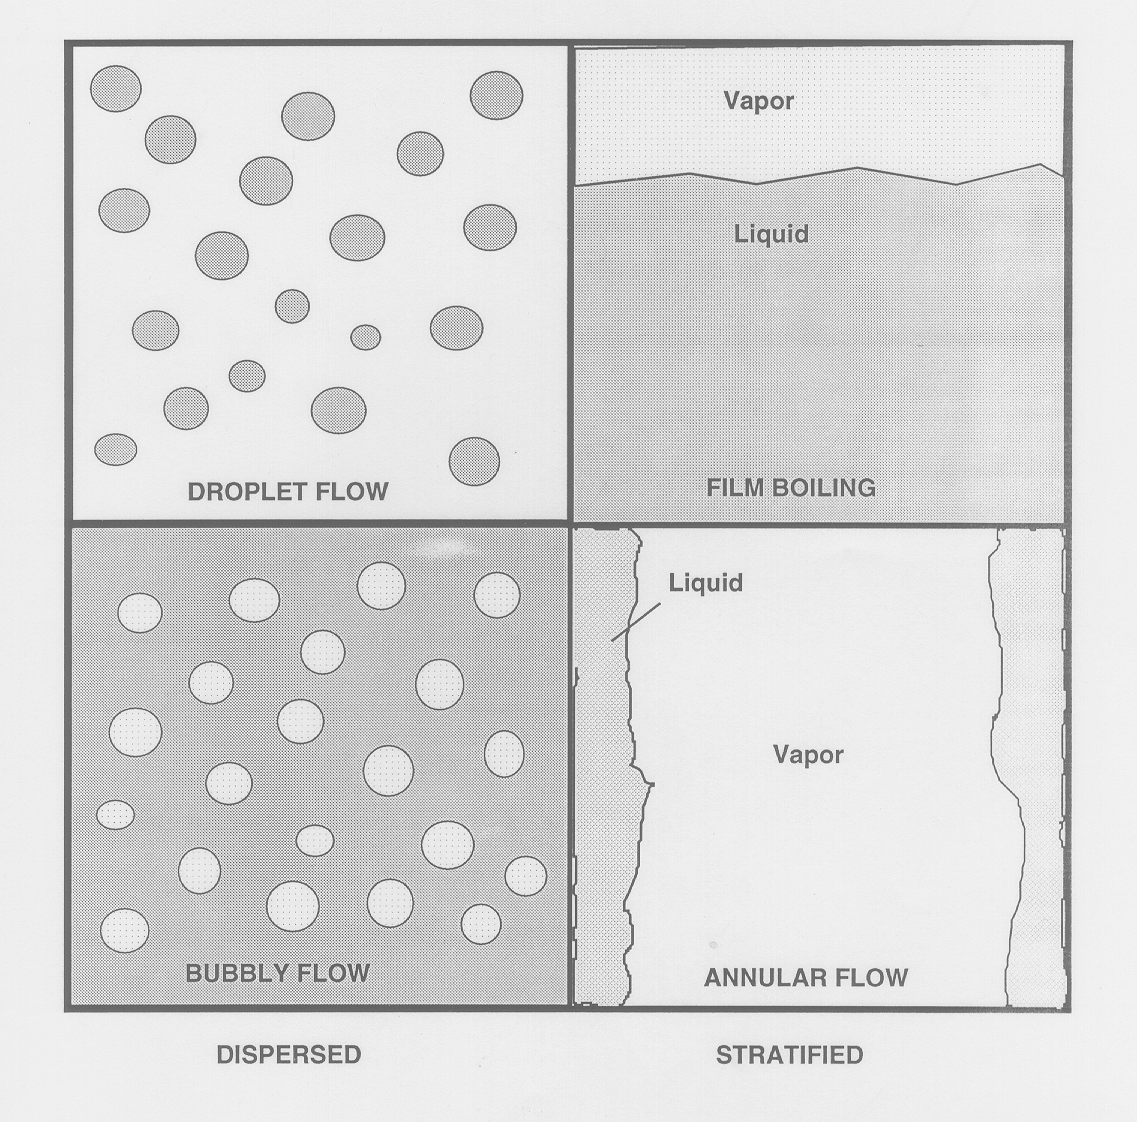
\includegraphics[width=0.95\textwidth]{images/general_flow_regime_map.png}
\caption{Gas-Liquid General Flow Regimes}
\label{fig:flow_regime_map}
\end{figure}

A dispersed flow pattern is one in which one or more phases are uniformly dispersed within a continuum of another phase with a length much smaller than the external scale; e.g., gas bubbles or solid particles in a liquid or liquid droplets in a gas or another immiscible liquid.
In this case the dispersed phase forms into nearly regular shaped particles with their stable size-governed again by a balance of buoyancy, inertial and surface tension forces.
The transitional flow regimes between these two fundamental types can take on may geometries.
Some of the more common transitional flow patterns are churn-turbulent and slug flow; i.e., dispersed-stratified flows where the discontinuous phase begins to form a continuum near the wall (bubbly-film) or in the center of the channel (wispy-annular).
These flow patterns will be discussed in more detail in a subsequent section.

\section{Pool Boiling}

One of the processes associated with a change in phase is evaporation.
This is simply the process of conversion of the liquid phase to vapor phase at an interface.
This process occurs whenever there is a concentration difference between the liquid phase and its vapor; e.g., water evaporation into the atmosphere of a room where the relative humidity is less than 100\%.

Boiling is the process in which a liquid evaporates and forms vapor pockets or regions within the continuous liquid phase.
Boiling can take many forms. Consider the common everyday occurrence of a pot of boiling water on top of the stove.
In this case a stagnant pool of liquid is heated and boiling occurs in the liquid at the bottom of the bulk liquid pool (Figure \ref{fig:pool_boiling}).
This overall process is called pool boiling. To form the vapor phase within the continuous liquid phase one must heat the liquid to a temperature above its saturation temperature, $T_{sat}$ ( $T_{sat}$ is that temperature at which the liquid exerts a vapor pressure equal to the ambient pressure).
If the temperature of the liquid rises far above $T_{sat}$ (e.g., \degreeC{210} for water), the vapor will be formed, "nucleate", as bubbles within the bulk of the liquid causing "volumetric" or "bulk" pool boiling.
This type of nucleation is termed "homogeneous nucleation" and is rarely observed in most common boiling situations.
Rather, if one were to look at the bottom of the pot of water on the stove one would notice the vapor bubbles nucleating at this heater surface.
In this case the temperature of the liquid does not need to be far above $T_{sat}$ (e.g., \degreeC{100} vs \degreeC{210} for water).
This nucleation occurs within "preferred-sites: or crevices within the heater surface aided by trapped vapor and gas is termed "heterogeneous nucleation".
This type of pool boiling is quite common in many industrial applications.

\begin{figure}[h!]
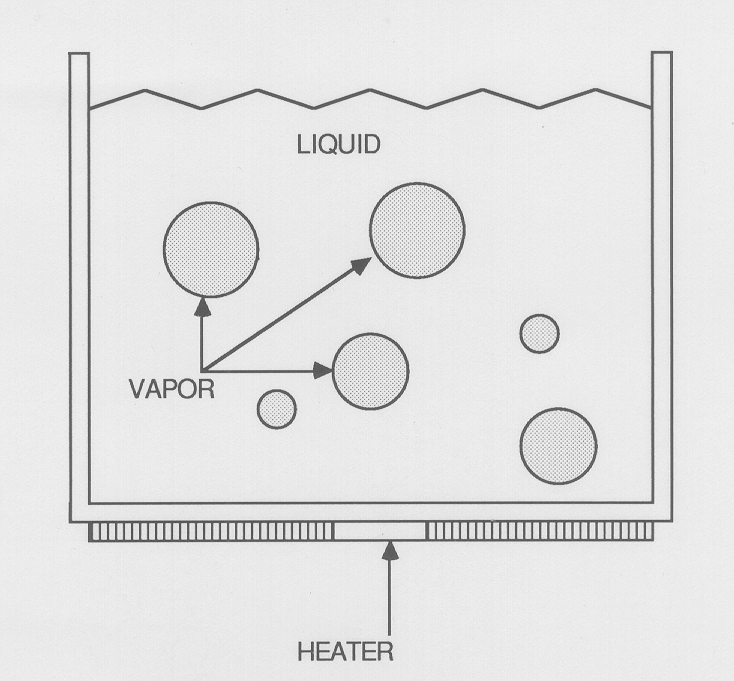
\includegraphics[width=0.5\textwidth]{images/pool_boiling.png}
\caption{Conceptual Picture of Pool Boiling}
\label{fig:pool_boiling}
\end{figure}

\section{Flow Boiling}

Flow boiling occurs when all the phases are in bulk flow together in a channel; e.g., vapor and liquid flow in a pipe.
The multiphase flow may be classified as adiabatic or diabatic, i.e., without or with heat addition at the channel wall (Figure \ref{fig:flow_boiling}).
An example of adiabatic flow would be oil/gas flow in a pipeline, or air/water flow.
In these cases the flow patterns would change as the inlet mass flow rates of the gas or liquid are altered or as the velocity and void distributions develop along the channel.
Boiling would not take place and phase change would only occur if in a one component multiphase flow (e.g., steam-water) the pressure decreases and flashing occurs.
Examples of diabatic flow are to be found in the riser tubes of steam generators and boiler tubes in power plants or in the coolant channels between nuclear fuel elements in a boiling water reactor.
Boiling occurs on the walls of the channels and the flow patterns change due to vapor production as one observes the flow downstream in the channel due to vapor production.
This is an important difference between pool boiling and flow boiling; i.e., that the forced flow of the multiphase system causes flow pattern transitions at a given wall heat flux (or temperature) as the integral power deposited in the fluid increases as it flows along the channel.

\begin{figure}[h]
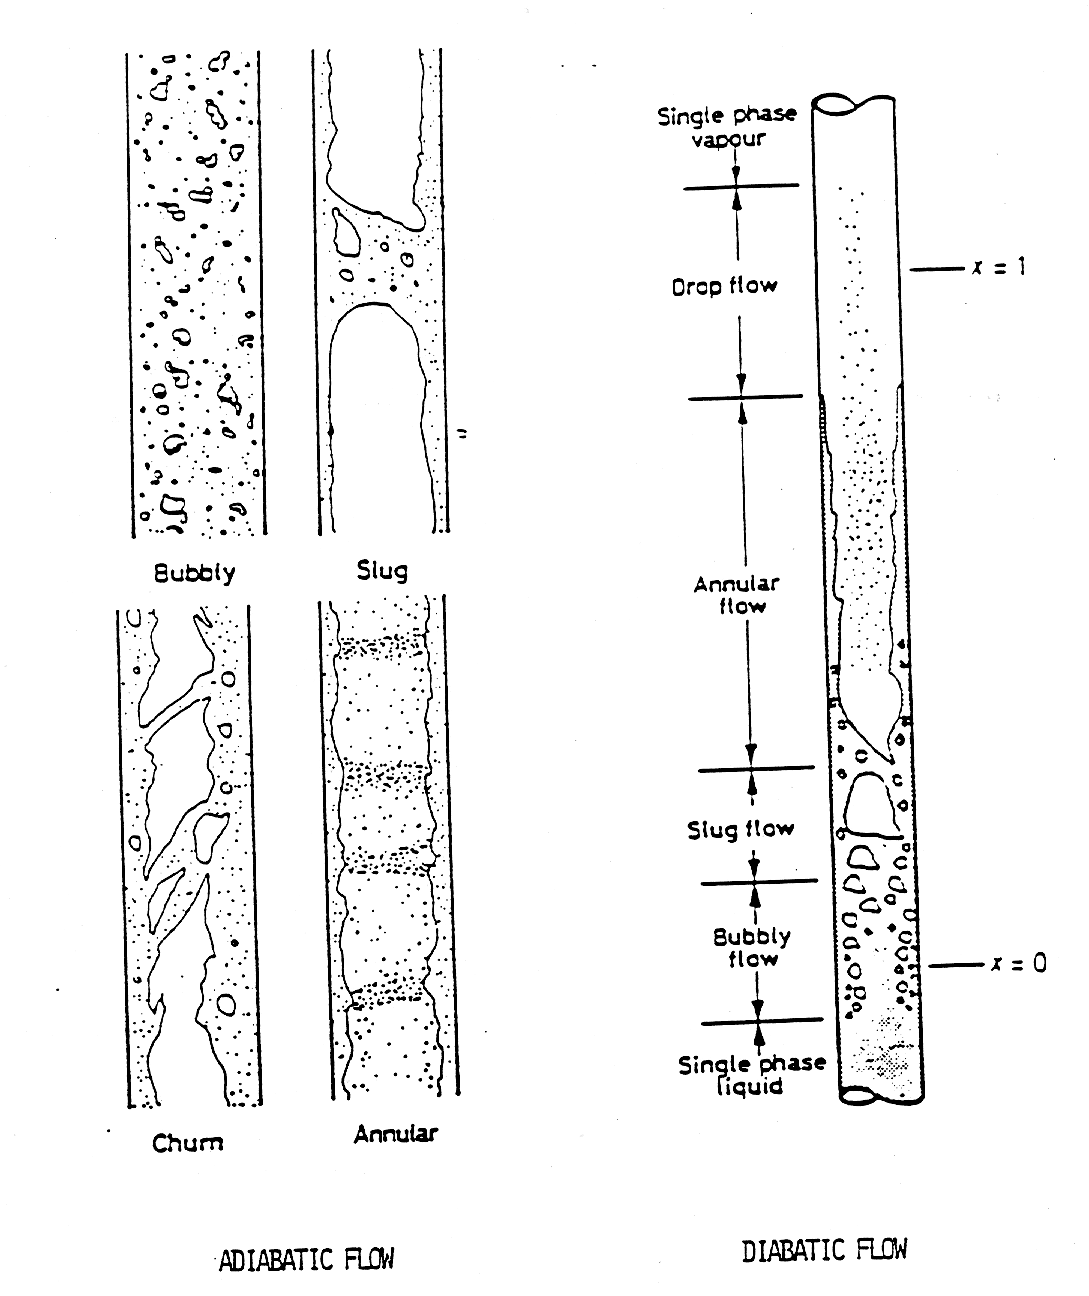
\includegraphics[width=0.5\textwidth]{images/flow_boiling.png}
\caption{Diabatic and Adiabatic Flow}
\label{fig:flow_boiling}
\end{figure}

In all cases of multiphase flow the velocities of the phases are usually not equal.
For example in a riser tube of a steam generator the vapor rises faster than the liquid due to buoyancy effects.
One may term this velocity inequality as "slip" between the vapor and the liquid.
The ratio of these velocities is called the "slip ratio".
A better description of the phenomena is to consider it as a relative velocity difference between the phases, $v_g - v_j$, and experimentally investigate these differences.
Flow boiling heat transfer can occur under two different boundary conditions, either a specified wall heat flux or a specified wall temperature.
The former case is an idealized example of a boiler tube in a fossil fuel boiler and the latter case is an idealized example of a riser tube in a steam generator.

\section{Condensation}

Condensation is the reverse process of evaporation; i.e., the process of conversion of vapor back into liquid.
It occurs when a wall (or the vapor near a wall) is cooled to a temperature which is below the saturation temperature corresponding to the vapor pressure.
This temperature is commonly called the dew point.
A common example of condensation occurs when steam condenses on the walls of the shower in a bathroom (Figure \ref{fig:condensation}).
Initially the water which condenses nucleates as droplets on the cold wall.
As the population of these droplets grow or the rate of condensation increases the droplets coalesce into a film which flows down the wall.
The first type of condensation is termed "dropwise" condensation and the second is termed "film" condensation. 
When the rate of condensation is low (e.g., a noncondensible gas is present) or when the liquid does not "wet" the wall, dropwise condensation occurs.
In most engineering components where condensation is a required part of an industrial process film condensation is expected, because of the large mass flux of condensed liquid per unit length of wetted area.

\begin{figure}[h]
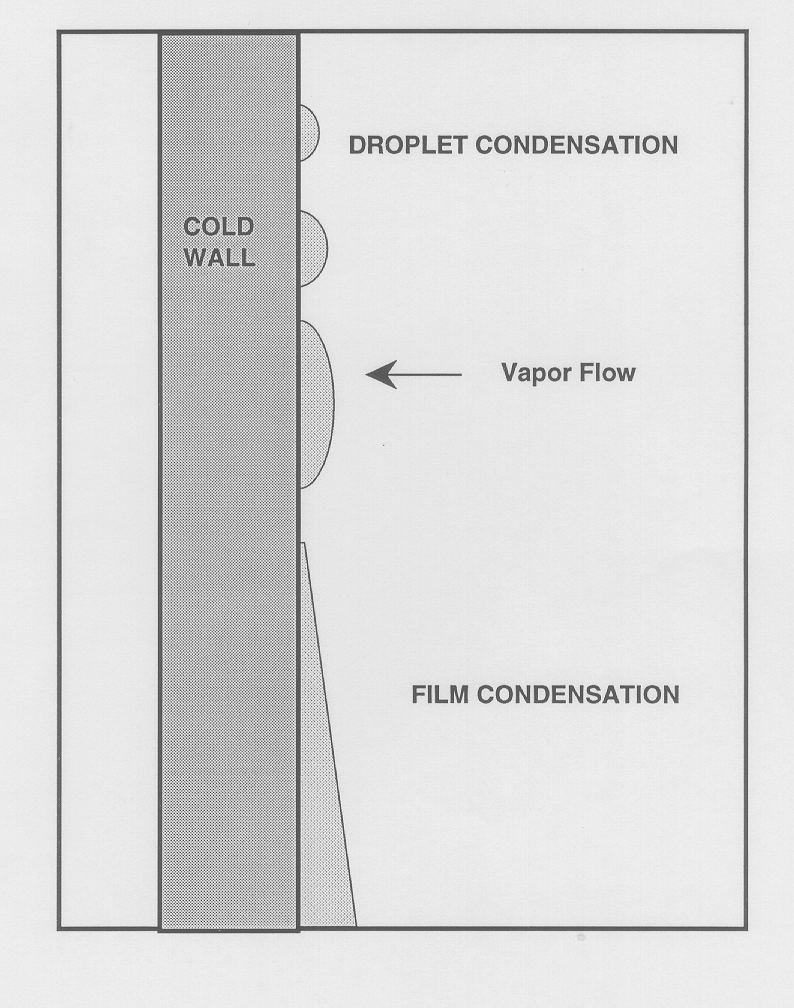
\includegraphics[width=0.5\textwidth]{images/condensation.png}
\caption{Conceptual Picture of Condensation}
\label{fig:condensation}
\end{figure}

Consider the temperature distribution through the vapor and liquid during condensation as shown in Figure \ref{fig:condensation}.
The temperature decreases in the vapor as one approaches the wall; appreciably if the vapor is superheated or if noncondensibles are present.
There is a slight decrease at the liquid-vapor interface due to the difference in pressure driving the mass transfer.
Also, there is a temperature drop in the liquid due to its thermal resistance to heat transfer.
If one were to plot the heat transfer coefficient as a function of distance down the wall one finds an interesting behavior.
Initially the heat transfer coefficient would decrease because more liquid accumulates as a film and acts as a thermal resistance.
However, at some liquid flow-rate the film becomes wavy and eventually turbulent.
This surface roughness actually reduces the thermal resistance in the flowing liquid film.
At this point and beyond the heat transfer increases as the liquid flow increases, with the Prandtl number having a second-order effect.
There are other effects which will be discussed later.